\DeclareMathAlphabet{\pazocal}{OMS}{zplm}{m}{n}
\newcommand{\Aa}{\mathcal{A}}
\newcommand{\Ab}{\pazocal{A}}

\section{Methodology}

% H transport model
\begin{equation}
    \frac{\partial c_\mathrm{m}}{\partial t}=\vec{\nabla} \cdot\left(D(T) \vec{\nabla}c_\mathrm{m}\right)+S-\sum \frac{\partial c_{\mathrm{t}, i}}{\partial t}
    \label{eq:mobile}
\end{equation}

\begin{equation}
    \frac{\partial c_{\mathrm{t}, i}}{\partial t}=k(T) \cdot c_\mathrm{m} \cdot\left(n_{i}-c_{\mathrm{t}, i}\right)-p(T) \cdot c_{\mathrm{t}, i}
    \label{eq:trapped}
\end{equation}

In Equation \ref{eq:mobile}, ${D(T)=D_0 \cdot \exp\big(-E_\mathrm{diff}/ (k_B \cdot T )\big)}$ is the diffusion coefficient in \si{m^2.s^{-1}}, $T$ the temperature in $\si{K}$ and ${k_B = 8.617 \times 10^{-5} \si{eV.K^{-1}}}$ the Boltzmann constant, $S$ is the volumetric source term of mobile particles in \si{m^{-3}.s^{-1}} (which can take into account plasma implantation), $k(T)=k_0\exp{\big(-E_{k} / (k_B \cdot T ) \big)}$ and $p(T)=p_0\exp{\big(-E_{p}/ (k_B \cdot T )\big)}$ are the trapping and detrapping rates expressed in \si{m^3.s^{-1}} and \si{s^{-1}} respectively.
$n_i$ is the trap density in \si{m^{-3}}.

% Bubbles trap density
Considering H is trapped on the surface of He bubbles, the equivalent trap density $n_b$ is given by:

\begin{equation}
    n_b = f \cdot c_b \cdot \Ab(\langle r_b \rangle)
\end{equation}
where $f$ is a free parameter representing the number of trapping site per unit surface, $\Ab = 4\pi \langle r_b \rangle^2$ is the area in \si{m^2} of a spherical bubble of radius $\langle r_b \rangle$, and $c_b$ is the concentration of bubbles in $\si{m^{-3}}$.


The radius of a bubble containing $\langle i_b \rangle$ He is given by:
\begin{equation}
    \begin{split}
        \langle r_b \rangle &= r(\mathrm{He}_{\langle i_b \rangle}\mathrm{V}_{\langle i_b \rangle/4}) \\
        &= r_{\mathrm{He}_0 \mathrm{V}_1} + \left(\frac{3}{4 \pi} \frac{a_0^3}{2} \frac{\langle i_b \rangle}{4} \right)^{1/3} - \left(\frac{3}{4 \pi} \frac{a_0^3}{2} \right)^{1/3}
    \end{split}
    \label{eq: radius average}
\end{equation}
with $a_0 = \SI{0.318}{nm}$ the lattice parameter and $r_{\mathrm{He}_0 \mathrm{V}_1} =  a_0 \sqrt{3}/4$.


The quantities $c_b$ and $\langle i_b \rangle$ have been computed from finite elements simulations \cite{delaporte-mathurin_influence_2021} (see Figure \ref{fig:trap bubbles distribution}).

\begin{figure}[h!]
    \centering
    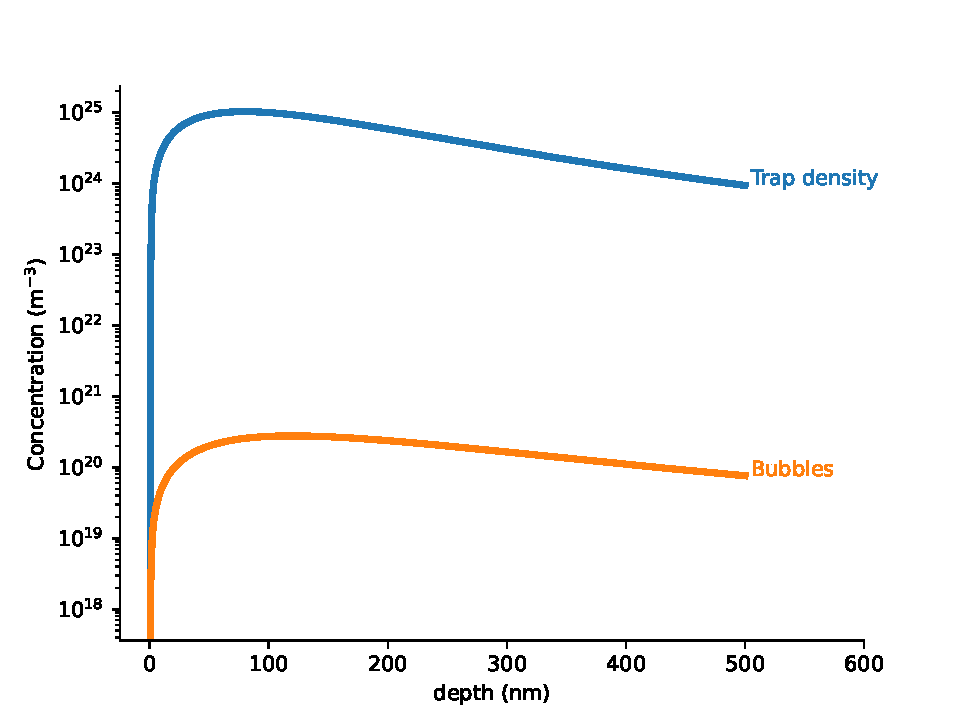
\includegraphics[width=\linewidth]{Figures/Chapter5/trap_bubble_distribution.pdf}
    \caption{Spatial distribution of the bubbles density and the equivalent trap density (assuming $f=\SI{3e18}{m^{-2}}$).}
    \label{fig:trap bubbles distribution}
\end{figure}

% Something describing Mykola's experiment
M Ialovega's experiment:
\begin{itemize}
    \item \cite{ialovega_hydrogen_2020}
\end{itemize}


% Describe the simulation problem
SIMULATION PROBLEM:
\begin{itemize}
    \item size of the sample: \SI{100}{\micro\metre}
    \item Diffusion coefficient $4.1\times 10 ^{-7} \exp{-0.39/k_B T}$ \cite{frauenfelder_solution_1969}
    \item  \SI{250}{eV} Deuterium: mean implantation depth \SI{10}{nm} width \SI{4.5}{nm} from SRIM \cite{ziegler_srim_2010}
    \item 4 traps are simulated (see Table \ref{tab: trap properties}) where some parameters are free (including the trapping sites surface density $f$)
    \item instantaneous recombination ($c_\mathrm{m} = 0$ at interfaces) is assumed
    \item Using the parametric optimisation method developed in \cite{delaporte-mathurin_parametric_2021} (14 degrees of freedom)
    \item simulated with FESTIM \cite{delaporte-mathurin_finite_2019}
\end{itemize} 

\begin{table}[!h]
    \caption{Trap properties used to fit the TDS spectra. The density distribution $n_b$ as well as detrapping energies $E_p$ are assumed constant across TDS experiments.}
    \begin{tabular}{r l l l l l}
    \\
     & $k_0$ & $E_k$ & $p_0$ & $E_p$ & $n$ \\
     \ & [\si{m^{3}.s{-1}}] & [\si{eV}] & [\si{s^{-1}}] & [\si{eV}] & [\si{m^{-3}}] \\
    \\
    Trap 1 & \multirow{7}{*} { $9 \times 10 ^{-17}$ } & \multirow{7}{*} { 0.39 } & \multirow{7}{*} { $10^{13}$ } & free & free \\
    \\
    Trap 2 & & & & free & free \\
    \\
    Trap 3 & & & & free & free \\
    \\
    Trap bubbles & & & & free & $n_b$ \\
    \end{tabular}
    \label{tab: trap properties}
\end{table}


\section{Results}

The properties obtained by the fitting procedure (see Table \ref{tab: trap properties results}) fitted well the three TDS spectra (see Figure \ref{fig: fitted TDS}).
As explained in \cite{ialovega_hydrogen_2020}, the last bump of desorption (around \SI{600}{K}) is due to a temperature control issue and was therefore ignored in the fitting procedure.
The detrapping energies of traps 1, 2 and 3 were found to be \SI{1.08}{eV}, \SI{1.20}{eV} and \SI{1.38}{eV} respectively, whereas the trap attributed to He bubbles has a detrapping energy of \SI{1.45}{eV}.


\begin{table}[!h]
    \caption{Results of the fitting procedure. Detrapping energies $E_p$ are given in \si{eV}, trap densities in \si{at.fr.} and $f$ in \si{m^{-2}}.}
    \begin{tabular}{r l l l l l l l l}
    \\
    &\multicolumn{2}{l}{Trap 1}  & \multicolumn{2}{l}{Trap 2} & \multicolumn{2}{l}{Trap 3} &\multicolumn{2}{l}{Trap bubbles} \\
     & $E_p$ & $n$ ($\times 10 ^{-3}$) & $E_p$ & $n$ ($\times 10 ^{-3}$) & $E_p$ & $n$ ($\times 10 ^{-3}$) & $E_p$ & $f$ ($\times 10 ^{18}$) \\
    \\
    1st TDS & - & 0.00 & - & 0.00 & - & 0.00 & 1.42 & $3.00$ \\
    \\
    2nd TDS & 1.08 & $2.20$ & 1.20 & $1.80$ & 1.37 & $2.00$ & 1.42 & $3.00$ \\
    \\
    5th TDS & 1.08 & $3.38$ & 1.20 & $3.10$ & 1.37 & $1.50$ & 1.42 & $3.00$ \\
    \end{tabular}
    \label{tab: trap properties results}
\end{table}

\begin{itemize}
    \item 1st He implantation: all pre-existing defects are saturated with He and bubbles are formed (proof from PAS that there are pre-existing defects before He implantation)
    \item 1st H implantation: H can only be trapped around bubbles since defects are saturated
    \item 1st TDS: H trapped around bubbles is desorbed (550K peak), He dissociates from HeV clusters (up to 1250K)
    \item 2nd H implantation: H is trapped around bubbles + in the non-saturated defects
    \item 2nd TDS: H trapped around bubbles is desorbed (550 K peak) + H trapped in non-saturated HeHV clusters (peaks 400K, 450K and 500K) + He trapped in deeper traps dissociate (TDS up to 1350K)
    
    \item 3rd to 5th implantation: H is trapped around bubbles + non-saturated defects
    \item 3rd to 5th TDS: H around bubbles is desorbed + more H dissociates from HeHV clusters
\end{itemize}




% After the first TDS, three additional peaks appear (traps 1, 2 and 3), which correlates with the fact that a small quantity of He left the sample after the first TDS.
% During all the following TDS cycles, the He desorption was much lower.
% This relates with the fact that the He bubbles traps density does not vary between the second and fifth TDS.
% The density of traps 1, 2 and 3 is increasing from the first TDS to the second.
% This suggests that some of the desorbed He was occupying defects such as vacancies.
% This attribution is also supported by the He TDS spectra shown in \cite{ialovega_hydrogen_2020}.
% These spectra showed that, during the first and second TDS, He desorbed at temperatures above \SI{1000}{K} which corresponds to $\mathrm{He}_m\mathrm{V}_1$ clusters \cite{faney_spatially_2014}.

This would mean that if the TDS were run up to temperature around \SI{1600}{K}, $\mathrm{He}_1\mathrm{V}_1$ clusters could dissociate resulting in additional free trapping sites for H and therefore different TDS spectra.

The H retention is not dominated by He-bubbles trapping but rather by secondary defects - potentially induced by the formation of bubbles.



\begin{figure}[h!]
    \centering
    \begin{subfigure}{\linewidth}
        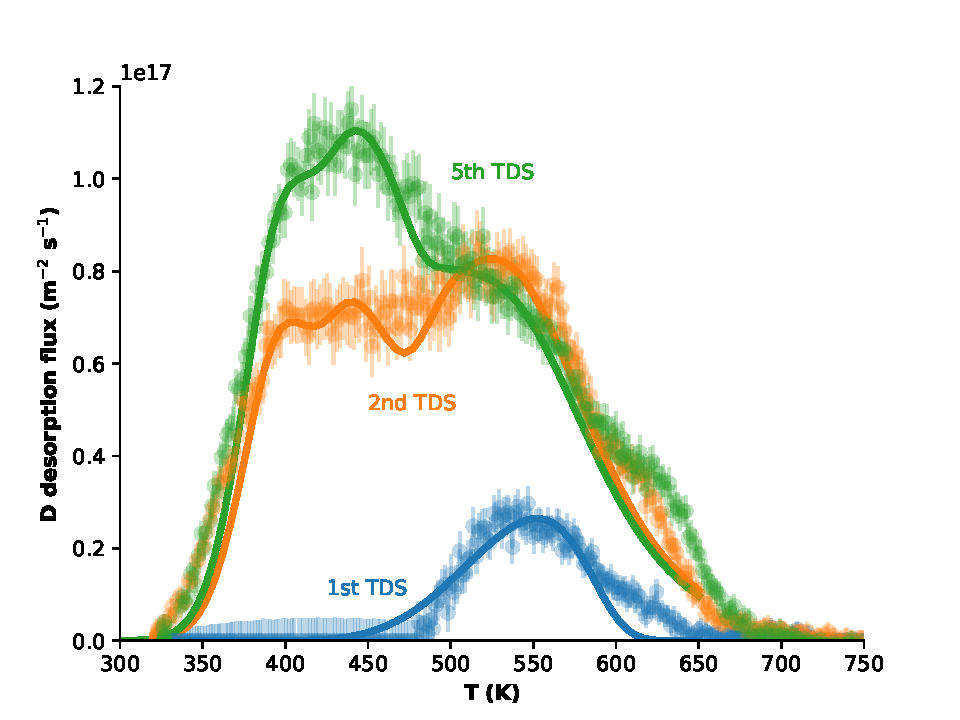
\includegraphics[width=\linewidth]{Figures/Chapter5/ialovega_tds.pdf}
        \caption{Experimental TDS spectra fitted with FESTIM}
        \label{fig: 3 TDS}
    \end{subfigure}
    \begin{subfigure}{\linewidth}
        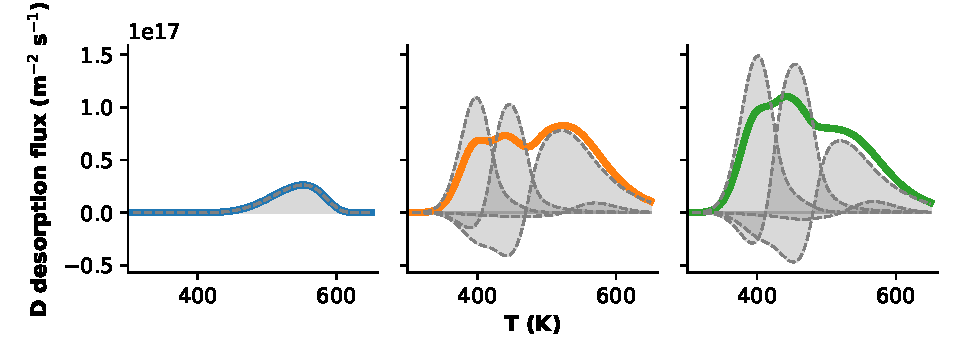
\includegraphics[width=\linewidth]{Figures/Chapter5/tds_trap_distribution.pdf}
        \caption{Traps contribution to the TDS spectra}
        \label{fig: trap contributions}
    \end{subfigure}
    \caption{Results of the TDS fitting procedure}
    \label{fig: fitted TDS}
\end{figure}

\begin{figure}
    \centering
    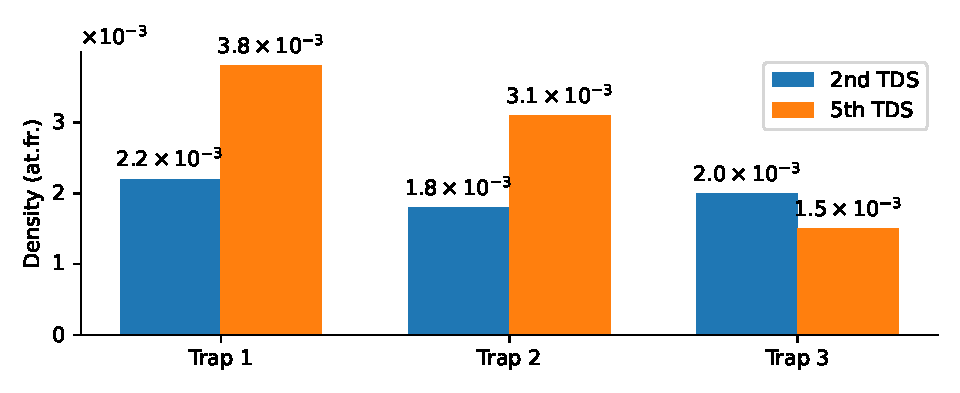
\includegraphics[width=\linewidth]{Figures/Chapter5/trap_densities.pdf}
    \caption{Caption}
    \label{fig:density evolution}
\end{figure}

The densities of traps 1 and 2 increased from the 2nd to the 5th TDS (see Figure \ref{fig:density evolution}).
However, the density of trap 3 decreased slightly (which is also visible on the TDS spectra shown in Figure \ref{fig: fitted TDS}).
This can be explained by either by 1) He leaving V-He complexes 2) annealing of some defects.
The processes at stake cannot yet be precisely described. 

\section*{Conclusion}

- H He implantation has been simulated with FESTIM
- One potential explanation of the effects observed in \cite{ialovega_hydrogen_2020}
- Though fitting a TDS spectrum is not sufficient to draw strong conclusions
- Suggests that 1) He doesn't leave bubbles in significant quantities at these temperatures 2) He occupies pre-existing defects avoiding H to get trapped 3) H retention is not dominated by He-induced bubbles

- Experimental suggestions: stop the TDS at \SI{750}{K} to limit He desorption. If the TDS spectra aren't affected this would confirm/infirm the He-induced trapping reduction effect.